
%(BEGIN_QUESTION)
% Copyright 2014, Tony R. Kuphaldt, released under the Creative Commons Attribution License (v 1.0)
% This means you may do almost anything with this work of mine, so long as you give me proper credit

Dette voltmeteret har et måleområde på 0 til 10 volt, og en indre resistans på 100k$\Omega$:

$$\includegraphics[width=10cm]{i01138x01.eps}$$

Vis hvordan vi kan øke måleområde til \textit{0 til 50} V, med å legge en motstand inn i kretsen. Regn også ut hvilken verdi denne motstanden  må ha og hvor stor effekt den må tåle. 

\underbar{file i01138}
%(END_QUESTION)





%(BEGIN_ANSWER)

The basic problem here is how to make the voltmeter see 10 volts while it's being connected to a source with a value of 50 volts.  This will require a {\it series} resistor to drop the extra 40 volts:

$$\includegraphics[width=15.5cm]{i01138x02.eps}$$

A power dissipation rating of ${1 \over 8}$ watt would be more than sufficient for this application.

%(END_ANSWER)





%(BEGIN_NOTES)

Voltmeter ranging is a very practical example of voltage divider circuitry.

%INDEX% Electronics review: series and parallel circuits

%(END_NOTES)


